\documentclass[11pt,letterpaper]{article}
\topmargin -.5truein
\textheight 9.0truein
\oddsidemargin 0truein
\evensidemargin 0truein
\textwidth 6.5truein
\setlength{\parskip}{5pt}
\setlength\parindent{0pt}
\usepackage[table]{xcolor}% http://ctan.org/pkg/xcolor
\usepackage{caption}
\usepackage{subcaption}
\usepackage[round]{natbib}
\usepackage{graphicx}
\usepackage{listings}
\usepackage{amsmath}
\usepackage{amssymb}
\usepackage{qtree}
\usepackage{algorithmic}
\usepackage{wrapfig}
\usepackage{tikz}
\usepackage{dsfont}
\usepackage{multirow}
\usepackage[all]{xy}
\usetikzlibrary{arrows,snakes,backgrounds,patterns,matrix,shapes,fit,calc,shadows,plotmarks}

\newcommand{\bs}{\textbackslash}
\renewcommand{\vec}[1]{\mathbf{#1}}

\newcommand{\ngramstart}{\ensuremath{\langle \textsc{s} \rangle}}
\newcommand{\ngramend}{\ensuremath{\langle \textsc{e} \rangle}}
\newcommand{\ngramunk}{\ensuremath{\langle unk \rangle}}

\usepackage{hyperref}
\hypersetup{
    colorlinks,
    citecolor=black,
    filecolor=black,
    linkcolor=black,
    urlcolor=black
}

\title{NLP: Hidden Markov Models}
\author{Dan Garrette\\\small{dhg@cs.utexas.edu}}

\begin{document}
\maketitle



\section{Tagging}

\begin{itemize}
  \item Named entities
  \item Parts of speech
\end{itemize}




\section{Parts of Speech}

Tagsets

\begin{itemize}
  \item Google Universal Tagset, 12: Noun, Verb, Adjective, Adverb, Pronoun, Determiner, Adposition (prepositions and postpositions), Numerals, Conjunctions, Particles, Punctuation, Other
  \item Penn Treebank, 45.  Includes 4 categores of noun, 4 categories of pronoun, and 6 categories of verb.
  \item Brown Corpus, 87
\end{itemize}

Deciding what categories

\begin{itemize}
  \item Auxilliary verbs?  ``I \textit{had} gone''
  \item Numbers as adjectives? ``I saw 4 cars''
  \item Count vs. mass nouns?  ``some apple'' vs. ``two apples'', ``some snow'' vs. ``two snows''
\end{itemize}

Uses

\begin{itemize}
  \item Parsing: determiner and noun should connect first, then to verb
  \item Speech synthesis: OBject (noun) vs. obJECT (verb), CONtent (noun) vs. conTENT (adj)
\end{itemize}

Rule-based

\begin{itemize}
  \item ``if it ends in `-tion' '' $\rightarrow$ Noun
  \item ``if it ends in `-ize' '' $\rightarrow$ Verb
  \item ``if it starts with `re-' '' $\rightarrow$ Verb
  \item ``if it starts with a capital letter'' $\rightarrow$ Proper Noun
  \item ``if it's preceded by `the' '' $\rightarrow$ Noun
  \item ``if it's followed by \textit{'s} '' $\rightarrow$ Noun
  \item ``if it's preceded by an adjective'' $\rightarrow$ Noun
  \item Or just memorize a big list of words and tags?
    \begin{itemize}
      \item Ambiguity?
      \item Picking the most common tag for a word $\rightarrow$ 90\% accuracy (thought state-of-the-art is 97\%)
    \end{itemize}
\end{itemize}

Open vs. Closed

\begin{itemize}
  \item Open class tags: new words are frequently added
    \begin{itemize}
      \item noun, verb, adjective, adverb
      \item ``Twitter'', to ``tweet'', ``twitterish''
    \end{itemize}
  \item Closed class tags: new words are rarely added
    \begin{itemize}
      \item determiner, preposition, pronouns, ...
      \item Don't want to completely close off new words
      \item Maybe \textit{alongside} (preposition) wasn't seen in training, only test
      \item New domains: ``u'' as a pronoun
    \end{itemize}
\end{itemize}

Complexitites:

\begin{itemize}
  \item Ambiguity:
    \begin{itemize}
      \item ``buy a book'' (noun) vs. ``book a flight'' (verb)
      \item ``talk over the deal'' (particle) vs. ``talk over the phone'' (prep)
    \end{itemize}
  \item Phrasal verbs: ``turn down'', ``rule out''
    \begin{itemize}
      \item ``he went on for days''
      \item ``he went on a boat''
    \end{itemize}
\end{itemize}



\section{Hidden Markov Models}


\begin{figure}[h]
\centering
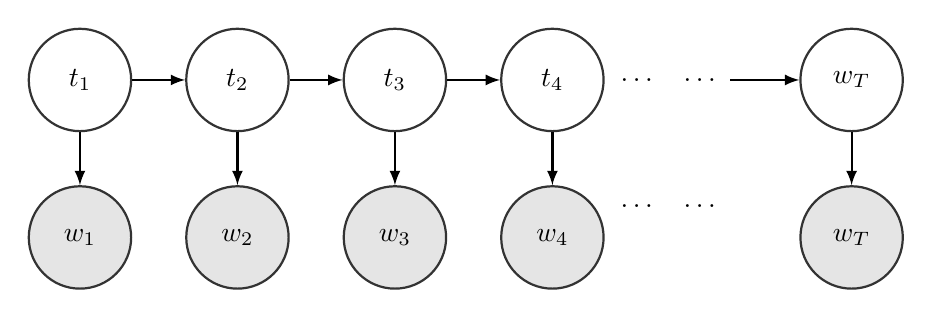
\begin{tikzpicture}
\tikzstyle{main}=[circle, minimum size = 13mm, thick, draw =black!80, node distance = 20mm]
\tikzstyle{obsv}=[main, fill = black!10]
\tikzstyle{hidden}=[node distance = 16mm]
\tikzstyle{connect}=[-latex, thick]
\tikzstyle{box}=[rectangle, draw=black!100]

  \node[main] (t1)                {$t_1$};
  \node[obsv] (w1) [below of =t1] {$w_1$};
  \node[main] (t2) [right of =t1] {$t_2$};
  \node[obsv] (w2) [below of =t2] {$w_2$};
  \node[main] (t3) [right of =t2] {$t_3$};
  \node[obsv] (w3) [below of =t3] {$w_3$};
  \node[main] (t4) [right of =t3] {$t_4$};
  \node[obsv] (w4) [below of =t4] {$w_4$};
  \node[hidden] (tI1) [right of =t4, xshift=-5mm] {$\dots$};
  \node[hidden] (wI1) [below of =tI1] {$\dots$};
  \node[hidden] (tI2) [right of =tI1, xshift=-8mm] {$\dots$};
  \node[hidden] (wI2) [below of =tI2] {$\dots$};
  \node[main] (tT) [right of=tI2, xshift=-1mm] {$w_T$};
  \node[obsv] (wT) [below of=tT] {$w_T$};

  \path (t1) edge [connect] (t2)
        (t2) edge [connect] (t3)
        (t3) edge [connect] (t4)
        (tI2) edge [connect] (tT)
        (t1) edge [connect] (w1)
        (t2) edge [connect] (w2)
        (t3) edge [connect] (w3)
        (t4) edge [connect] (w4)
        (tT) edge [connect] (wT);

\end{tikzpicture}
\caption{Second-order HMM showing conditional dependencies}
\end{figure} 

\begin{figure}[h]
\centering
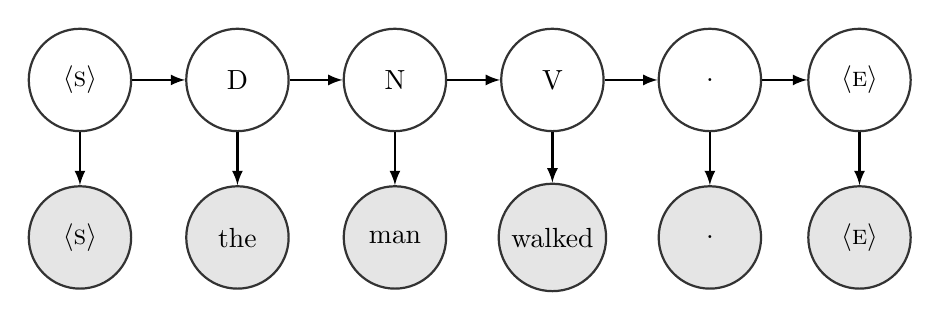
\begin{tikzpicture}
\tikzstyle{main}=[circle, minimum size = 13mm, thick, draw =black!80, node distance = 20mm]
\tikzstyle{obsv}=[main, fill = black!10]
\tikzstyle{hidden}=[node distance = 16mm]
\tikzstyle{connect}=[-latex, thick]
\tikzstyle{box}=[rectangle, draw=black!100]

  \node[main] (t1)                {\ngramstart};
  \node[obsv] (w1) [below of =t1] {\ngramstart};
  \node[main] (t2) [right of =t1] {D};
  \node[obsv] (w2) [below of =t2] {the};
  \node[main] (t3) [right of =t2] {N};
  \node[obsv] (w3) [below of =t3] {man};
  \node[main] (t4) [right of =t3] {V};
  \node[obsv] (w4) [below of =t4] {walked};
  \node[main] (t7) [right of =t4] {.};
  \node[obsv] (w7) [below of =t7] {.};
  \node[main] (tT) [right of =t7, xshift=-1mm] {\ngramend};
  \node[obsv] (wT) [below of =tT] {\ngramend};

  \path (t1) edge [connect] (t2)
        (t2) edge [connect] (t3)
        (t3) edge [connect] (t4)
        (t4) edge [connect] (t7)
        (t7) edge [connect] (tT)

        (t1) edge [connect] (w1)
        (t2) edge [connect] (w2)
        (t3) edge [connect] (w3)
        (t4) edge [connect] (w4)
        (t7) edge [connect] (w7)
        (tT) edge [connect] (wT);

\end{tikzpicture}
\caption{Second-order HMM for the sentence ``the man walks .''}
\end{figure} 



Similar to N-Gram models

\begin{itemize}
  \item Model the text as a \textit{sequence}
    \begin{itemize}
      \item Bad assumption, but less sparse
    \end{itemize}
  \item For ngrams, we modeled the probability of each word conditioned on the previous n-1 words.
  \item Here, we model each \textit{tag} conditioned on previous \textit{tags}
  \item Still uses Markov assumption: only look back a few tags
    \begin{itemize}
      \item Again, bad assumption, but less sparse
    \end{itemize}
  \item Note that we have to condition words on tags because otherwise 
\end{itemize}


~\\ \bs\bs~ Day 2 \\

Derivation

\begin{itemize}
  \item We want the most likely tag sequence for a sequence of words: \vspace{2mm} \\
        $~~~~~~~~~~p(\ngramstart~t_1~t_2~...~t_n~\ngramend \mid \ngramstart~w_1~w_2~...~w_n~\ngramend)$
        \vspace{2mm} \\ Remember that order matters!
  \item For simplicity, we'll write this as $t_1^n = \langle t_1, t_2, ..., t_n \rangle$
  \item So we want  \vspace{2mm} \\
  $~~~~~~~~~~~~~\hat{t}_1^n = \text{argmax}_{t_1^n}~p(\ngramstart~t_1~t_2~...~t_n~\ngramend \mid \ngramstart~w_1~w_2~...~w_n~\ngramend)$ \vspace{2mm} \\ but it's hard to estimate
  \item Like for ngrams, use Bayes rule: 
  \begin{align*}
  \hat{t}_1^n 
  &= \text{argmax}_{t_1^n}~\frac{p(\ngramstart~w_1~w_2~...~w_n~\ngramend \mid \ngramstart~t_1~t_2~...~t_n~\ngramend) \cdot p(\ngramstart~t_1~t_2~...~t_n~\ngramend}{p(\ngramstart~w_1~w_2~...~w_n~\ngramend)} \\
  & = \text{argmax}_{t_1^n}~p(\ngramstart~w_1~w_2~...~w_n~\ngramend \mid \ngramstart~t_1~t_2~...~t_n~\ngramend) \cdot p(\ngramstart~t_1~t_2~...~t_n~\ngramend)
\end{align*}

  \item Two major independence assumptions:
    \begin{itemize}
      \item Like ngrams, assume probability of a sequence is dependent only on recent past:
        \begin{align*}
          p(\ngramstart~t_1~t_2~...~t_n~\ngramend) 
                    &\approx p(t_1 \mid \ngramstart) \cdot 
                              p(t_2 \mid t_1) \cdot 
                              p(t_2 \mid t_2) \cdot 
                              ...  \cdot 
                              p(t_n \mid t_{n-1}) \cdot 
                              p(\ngramend \mid t_n) \\
                    &= \prod_{i=1}^n p(t_i \mid t_{i-1})
        \end{align*}
      \item Also assume word is only dependent on its tag: \vspace{2mm}
        \begin{align*}
          p(\ngramstart~w_1~w_2~...~w_n~\ngramend \mid \ngramstart~t_1~t_2~...~t_n~\ngramend) 
                    &\approx p(w_1 \mid t_1) \cdot 
                             p(w_2 \mid t_2) \cdot 
                             ...  \cdot 
                             p(w_n \mid t_n) \\
                    &= \prod_{i=1}^n p(w_i \mid t_i)
        \end{align*}
      \item Together: 
        \begin{align*}
        \hat{t}_1^n &= \text{argmax}_{t_1^n}~p(\ngramstart~t_1~t_2~...~t_n~\ngramend \mid \ngramstart~w_1~w_2~...~w_n~\ngramend) \\
                    &= \text{argmax}_{t_1^n}~p(\ngramstart~w_1~w_2~...~w_n~\ngramend \mid \ngramstart~t_1~t_2~...~t_n~\ngramend) \cdot p(\ngramstart~t_1~t_2~...~t_n~\ngramend) \\
                    &\approx \text{argmax}_{t_1^n}~\prod_{i=1}^n p(w_i \mid t_i) \cdot p(t_i \mid t_{i-1})
        \end{align*}
    \end{itemize}
\end{itemize}


\section{Estimating Parameters: MLE}

Two probability distributions to estimate:

\begin{itemize}
  \item Transitions: probability of a tag, given previous tag, $p(t_i \mid t_{i-1})$
  \item Emissions: probability of a word, given its tag, $p(w_i \mid t_i)$
\end{itemize}

MLE

\begin{itemize}
  \item MLE estimation is just like before (na\"{i}ve Bayes, ngrams, ...), normalized counts
  \item Transitions: $p(t_i \mid t_{i-1}) = \frac{C(t_{i-1}~t_i)}{\sum_x C(t_{i-1}~x)} = \frac{C(t_{i-1}~t_i)}{C(t_{i-1})}$
  \item Emissions: $p(w_i \mid t_i) = \frac{C(t_i,w_i)}{\sum_x C(t_i,x)} = \frac{C(t_i,w_i)}{C(t_i)}$
\end{itemize}

Example dataset:
\vspace{-2mm}
\begin{verbatim}
    <S>|<S> the|D man|N walks|V the|D dog|N .|. <E>|<E> 
    <S>|<S> the|D dog|N runs|V .|. <E>|<E> 
    <S>|<S> the|D dog|N walks|V .|. <E>|<E> 
    <S>|<S> the|D man|N walks|V .|. <E>|<E> 
    <S>|<S> a|D man|N saw|V the|D dog|N .|. <E>|<E> 
    <S>|<S> the|D cat|N walks|V .|. <E>|<E> 
\end{verbatim}

Some probabilities:

\begin{itemize}
  \item $p(t_i=\text{V} \mid t_{i-1}=\text{N}) = \frac{C(\text{N V})}{\sum_x C(\text{N } x)} = \frac{6}{8} = 0.75$
  \item $p(t_i=\text{D} \mid t_{i-1}=\text{N}) = \frac{C(\text{N D})}{\sum_x C(\text{N } x)} = \frac{0}{8} = 0.0$
  \\
  \item $p(w_i=\text{dog} \mid t_i=\text{N}) = \frac{C(\text{N,dog})}{\sum_x C(\text{N},x)} = \frac{4}{8} = 0.50$
  \item $p(w_i=\text{the} \mid t_i=\text{N}) = \frac{C(\text{N,the})}{\sum_x C(\text{N},x)} = \frac{0}{8} = 0.0$
\end{itemize}


\section{Add-$\lambda$ Smoothing}

\begin{itemize}
  \item Again, just like before.
  \item Transitions: $p(t_i \mid t_{i-1}) 
             = \frac{C(t_{i-1}~t_i)+\lambda}{\sum_x (C(t_{i-1}~x)+\lambda)} 
             = \frac{C(t_{i-1}~t_i)+\lambda}{(\sum_x C(t_{i-1}~x))+\lambda\cdot|T|} 
             = \frac{C(t_{i-1}~t_i)}{C(t_{i-1})}$
  \item Emissions: $p(w_i \mid t_i) 
             = \frac{C(t_i,w_i)+\lambda}{\sum_x (C(t_i,x)+\lambda)} 
             = \frac{C(t_i,w_i)+\lambda}{(\sum_x C(t_i,x))+\lambda\cdot|V|} 
             = \frac{C(t_i,w_i)}{C(t_i)}$
\end{itemize}

Some probabilities (with $\lambda=2$):

\begin{itemize}
  \item $V = \{ a, cat, dog, man, runs, saw, the, walks, ., \ngramend \}$, ~~$|V|=10$   \vspace{2mm} \\
        $T = \{ D, N, V, \ngramend \}$, ~~$|N|=4$
  \\
  \item $p(t_i=\text{V} \mid t_{i-1}=\text{N}) 
     = \frac{C(\text{N V})+2}{\sum_x (C(\text{N } x)+2)} 
     = \frac{C(\text{N V})+2}{(\sum_x C(\text{N } x))+(2 \cdot 4)} 
     = \frac{6+2}{8+8} = 0.75
     = \frac{8}{16} = 0.50$
  \item $p(t_i=\text{D} \mid t_{i-1}=\text{N}) 
     = \frac{C(\text{N D})+2}{\sum_x (C(\text{N } x)+2)} 
     = \frac{C(\text{N D})+2}{(\sum_x C(\text{N } x))+(2 \cdot 4)} 
     = \frac{0+2}{8+8}
     = \frac{2}{16} = 0.125$
  \\
  \item $p(w_i=\text{dog} \mid t_i=\text{N}) 
     = \frac{C(\text{N,dog})}{\sum_x (C(\text{N},x)+2)} 
     = \frac{C(\text{N,dog})}{(\sum_x C(\text{N},x))+(2 \cdot 10)} 
     = \frac{4+2}{8+10}
     = 0.33$
  \item $p(w_i=\text{the} \mid t_i=\text{N}) 
     = \frac{C(\text{N,the})}{\sum_x (C(\text{N},x)+2)} 
     = \frac{C(\text{N,the})}{(\sum_x C(\text{N},x))+(2 \cdot 10)} 
     = \frac{0+2}{8+10} 
     = 0.11$
\end{itemize}

Differences:

\begin{itemize}
  \item Two distributions, two kinds of smoothing
  \item Can do add-$\lambda$ for both, but don't need to use same $\lambda$
  \item Can use totally different smoothing for each.
\end{itemize}





\section{Decoding}

Tagging a sentence

\begin{itemize}
  \item $\text{argmax}_{t_1^n}~\prod_{i=1}^n p(w_i \mid t_i) \cdot p(t_i \mid t_{i-1})$
  \item For ``the dog walks .'', we have to check all combinations: \vspace{2mm} \\
        \ngramstart\ D D D D \ngramend  \vspace{2mm} \\
        \ngramstart\ N D D D \ngramend  \vspace{2mm} \\
        \ngramstart\ V D D D \ngramend  \vspace{2mm} \\
        \ngramstart\ . D D D \ngramend  \vspace{2mm} \\
        \ngramstart\ N N D D \ngramend  \vspace{2mm} \\
        \ngramstart\ N V D D \ngramend  \vspace{2mm} \\
        ...
  \item But this is insane.
\end{itemize}

Choosing a tag

\begin{itemize}
  \item Because of our independence assumptions, the probability of each tag is dependent only on its ``Markov blanket''
  \item Look only at the previous tag, emitted word, and next tag.  
    \begin{align*} p(t_i \mid \ngramstart~w_1~w_2~...~w_n~\ngramend, \ngramstart~t_1~t_2~...~\mathbf{t_{i-1}~t_{i+1}}~...~t_n~\ngramend)
       &= p(t_i \mid t_{i-1}, w_i, t_{i+1}) \\
       &= p(t_i \mid t_{i-1}) \cdot p(w_i \mid t_i) \cdot p(t_{i+1} \mid t_i)
    \end{align*}
\end{itemize}

Tagging a sentence

\begin{itemize}
  \item We want to make global decisions about tags.
  \item Due to independence, global decisions are made in terms of local decisions
  \item Going ``forward'' allows us to predict tags based on previous decisions.
  \item But we can't calculate picking a tag changes the probabilities of previous tags.
\end{itemize}

Dynamic Programming:

\begin{itemize}
  \item We need to check all possible tag combinations \textit{efficiently}
  \item 
\end{itemize}


\begin{align}
P(s_t=k | y_{1:t}) &=  
P(y_t | k) \cdot \sum_{k' \in K} P(k|k') \cdot P(s_{t-1}=k' | y_{1:t-1})
\end{align}

\begin{align}
P(s_t=k | s_{t+1}, y_{1:T}) &\propto
P(s_t=k | y_{1:t}) \cdot P(s_{t+1} | s_t=k)
\end{align}




Tag the sentence: ``the dog runs .''

% \begin{align*}

% \end{align*}



\section{Tag Dictionary}

\begin{itemize}
  \item Mapping from words to potential tags
  \item Get from train, assume works on test
  \item Unseen words usually assumed to be any possible tag.  Could, instead, assume only open-class tags.
  \item Prune low-probability tags
\end{itemize}







\newsavebox{\starttable}
\sbox{\starttable}{
    \begin{tabular}{l l}
      \hline
      \multicolumn{2}{|c|}{{\cellcolor{gray!40}\ngramstart}} \tabularnewline
      \hline
      \ngramstart & 1.0
    \end{tabular}
}

\newsavebox{\Dtable}
\sbox{\Dtable}{
    \begin{tabular}{l l}
      \hline
      \multicolumn{2}{|c|}{{\cellcolor{gray!40}D}} \tabularnewline
      \hline
      the & 0.87 \tabularnewline
      a   & 0.13
    \end{tabular}
}

\newsavebox{\Ntable}
\sbox{\Ntable}{
    \begin{tabular}{l l}
      \hline
      \multicolumn{2}{|c|}{{\cellcolor{gray!40}N}} \tabularnewline
      \hline
      man & 0.25 \tabularnewline
      dog & 0.50 \tabularnewline
      cat & 0.25
    \end{tabular}
}

\newsavebox{\Vtable}
\sbox{\Vtable}{
    \begin{tabular}{l l}
      \hline
      \multicolumn{2}{|c|}{{\cellcolor{gray!40}V}} \tabularnewline
      \hline
      walks  & 0.66 \tabularnewline
      runs   & 0.17 \tabularnewline
      chases & 0.17
    \end{tabular}
}

\newsavebox{\stoptable}
\sbox{\stoptable}{
    \begin{tabular}{l l}
      \hline
      \multicolumn{2}{|c|}{{\cellcolor{gray!40}.}} \tabularnewline
      \hline
      . & 1.0
    \end{tabular}
}

\newsavebox{\ngramendtable}
\sbox{\ngramendtable}{
    \begin{tabular}{l l}
      \hline
      \multicolumn{2}{|c|}{{\cellcolor{gray!40}\ngramend}} \tabularnewline
      \hline
      \ngramend & 1.0
    \end{tabular}
}


\begin{figure}[h]
\centering
\begin{tikzpicture}
\tikzstyle{main}=[rectangle, thick, draw =black!80, node distance = 40mm]
\tikzstyle{obsv}=[main, fill = black!10]
\tikzstyle{hidden}=[node distance = 16mm]
\tikzstyle{connect}=[-latex, thick]
\tikzstyle{box}=[rectangle, draw=black!100]

  \node[main] (start) []           {\usebox{\starttable}};
  \node[main] (D)     [right of =start]          {\usebox{\Dtable}};
  \node[main] (N)     [right of =D, yshift= 70]  {\usebox{\Ntable}};
  \node[main] (V)     [right of =D, yshift=-70]  {\usebox{\Vtable}};
  \node[main] (stop)  [right of =D, xshift=40mm] {\usebox{\stoptable}};
  \node[main] (end)   [right of =stop]           {\usebox{\ngramendtable}};


  \path (start) edge [connect] node [pos=0.5, above, blue, sloped] {1.0} (D);
  \path (D) edge [connect] node [pos=0.5, above, blue, sloped] {1.0} (N);
  \path (N) edge [connect] node [pos=0.5, above, blue, sloped] {0.80} (V);
  \path (N) edge [connect] node [pos=0.5, above, blue, sloped] {0.20} (stop);
  \path (V) edge [connect, red] node [pos=0.5, above, blue, sloped] {0.33} (D);
  \path (V) edge [connect] node [pos=0.5, above, blue, sloped] {0.67} (stop);
  \path (stop) edge [connect] node [pos=0.5, above, blue, sloped] {1.0} (end);
  

\end{tikzpicture}
\caption{Finite state machine.  Missing arrows are assumed to be zero probabilities.  With smoothing, there would be an arrow in \textit{both directions} between \textit{every} pair of words.}
\end{figure} 






\end{document}

